\documentclass[border=2pt]{standalone}
\usepackage[T1]{fontenc}
\usepackage{mathptmx}
\usepackage{amsmath,amssymb}
\usepackage{tikz}
\usetikzlibrary{arrows.meta,positioning,calc}
\begin{document}
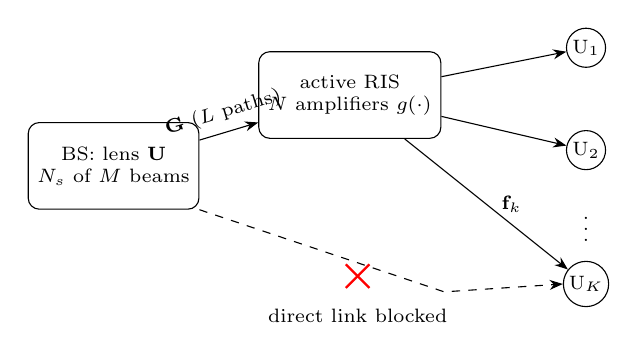
\begin{tikzpicture}[x=1cm,y=1cm,>=Stealth,font=\scriptsize,every node/.style={align=center}]
\node[draw,rounded corners,minimum width=1.6cm,minimum height=1.1cm] (bs) at (0,0) {BS: lens $\mathbf U$\\ $N_s$ of $M$ beams};
\node[draw,rounded corners,minimum width=1.7cm,minimum height=1.1cm] (ris) at (3.0,0.9) {active RIS\\ $N$ amplifiers $g(\cdot)$};
\node[draw,circle,inner sep=1pt] (u1) at (6.0,1.5) {U$_1$};
\node[draw,circle,inner sep=1pt] (u2) at (6.0,0.2) {U$_2$};
\node (u3) at (6.0,-0.7) {$\vdots$};
\node[draw,circle,inner sep=1pt] (uK) at (6.0,-1.5) {U$_K$};
\draw[->] (bs) -- node[above,sloped]{$\mathbf G\ (L$ paths)} (ris);
\draw[->] (ris) -- (u1); \draw[->] (ris) -- (u2); \draw[->] (ris) -- node[right,xshift=2pt]{$\mathbf f_k$} (uK);
\draw[dashed,->] (bs.south east) -- (4.2,-1.6) -- (uK.west);
\node at (3.1,-1.9) {direct link blocked};
\draw[red,thick] (2.95,-1.25) -- (3.25,-1.55); \draw[red,thick] (3.25,-1.25) -- (2.95,-1.55);
\end{tikzpicture}
\end{document}
